\section{Entscheidungsprozesse}

\begin{frame}[c]{Fehlerquellen in Entscheidungsprozessen}
    \centering
    % Folie langsam aufbauen, ist sonst zu viel information auf einmal
    % Konkretes Beispiel!!
    % ideen: Kaufen eines Produktes im Supermarkt
    % idee: Terminoptimierung - Freizeitoption A oder B, fokus auf Gruppendynamik
    % \only<1>{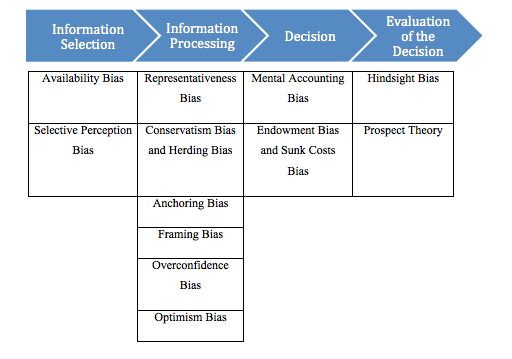
\includegraphics[width=\textwidth, clip=true, trim= 0mm 102mm 0mm 0mm]{DecisionMakingProcedure}}
    \only<1->{
\includegraphics[width=\textwidth]{DecisionMakingProcedure0}\vfill}
%     \only<2>{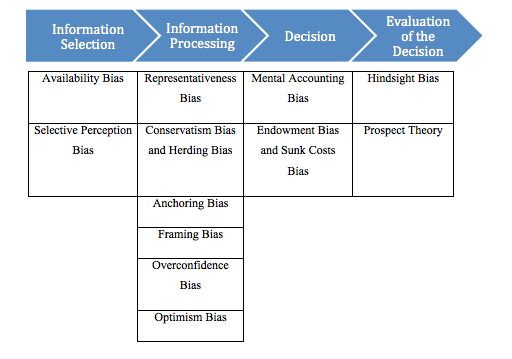
\includegraphics[width=\textwidth]{DecisionMakingProcedure}}
\end{frame}

\begin{frame}[c]{Entscheidungsprozesse - Beispiel}
    \Large
    Situation: Man möchte ein neues Handy kaufen. \\
\end{frame}


\begin{frame}[c]{Kaufen eines neuen Handys}
    
\includegraphics[width=\textwidth]{Sammeln_Informationen} \\
    \pause
    Hier müssen wir vor allem aufpassen bezüglich:
    \begin{itemize}[<+(1)->]
        \item Verzerrungen der Verfügbarkeit
            % Jemand hat erst am Tag zuvor ein Handy empfohlen vs Länger zuvor
        \item Selektiver Wahrnehmung
            % Die Tendenz, genau das zu sehen das man sehen möchte
        \item Bestätigungsvoreingenommenheit
            % Man sucht, interpretiert und beschäftigt sich hauptsächlich mit bestätigenden informationen
        \item Frequenzillusion
            % Frequenzen werden üblicherweise unverständlich dargestellt
    \end{itemize}
    (von Informationen)
\end{frame}


\begin{frame}[c]{Kaufen eines neuen Handys}
    
\includegraphics[width=\textwidth]{Informations_Verarbeitung} \\
    \pause
    Hier müssen wir vor allem aufpassen bezüglich:
    \begin{itemize}[<+(1)->]
        \item Repräsentativität
        \item Ankereffekt/Rahmungseffekt
        \item Optimismus/Übersteigertes Selbstvertrauen
        \item Gruppenzwang
        \item Konservativität
    \end{itemize}
\end{frame}


\begin{frame}[c]{Kaufen eines neuen Handys}
    
\includegraphics[width=\textwidth]{Entscheidung} \\
    \pause
    Hier müssen wir vor allem aufpassen bezüglich:
    \begin{itemize}[<+(1)->]
        \item Schubladendenken (Mental Accounting Bias)
        \item Besitztum (Endowment Bias)
        \item Täuschung der investierten Kosten
        \item Wählen des Üblichen
        \item Gesetz des Instruments
    \end{itemize}
\end{frame}


\begin{frame}[c]{Kaufen eines neuen Handys}
    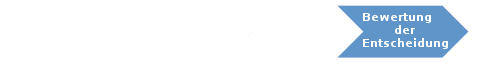
\includegraphics[width=\textwidth]{Bewertung} \\
    \pause
    Hier müssen wir vor allem aufpassen bezüglich:
    \begin{itemize}[<+(1)->]
        \item Rückschaufehler (Hindsight)
        \item Verantwortung (Self-Serving bias)
        \item Gültigkeitsillusion (Illusion of validity)
        \item Fokussierung
        \item Nachträgliche Begründungstendenz
    \end{itemize}
\end{frame}




\begin{frame}[standout]
    ... und das ist nur ein kleiner Auszug.
\end{frame}

\begin{frame}[c]{List of cognitive Biases}
    \centering
    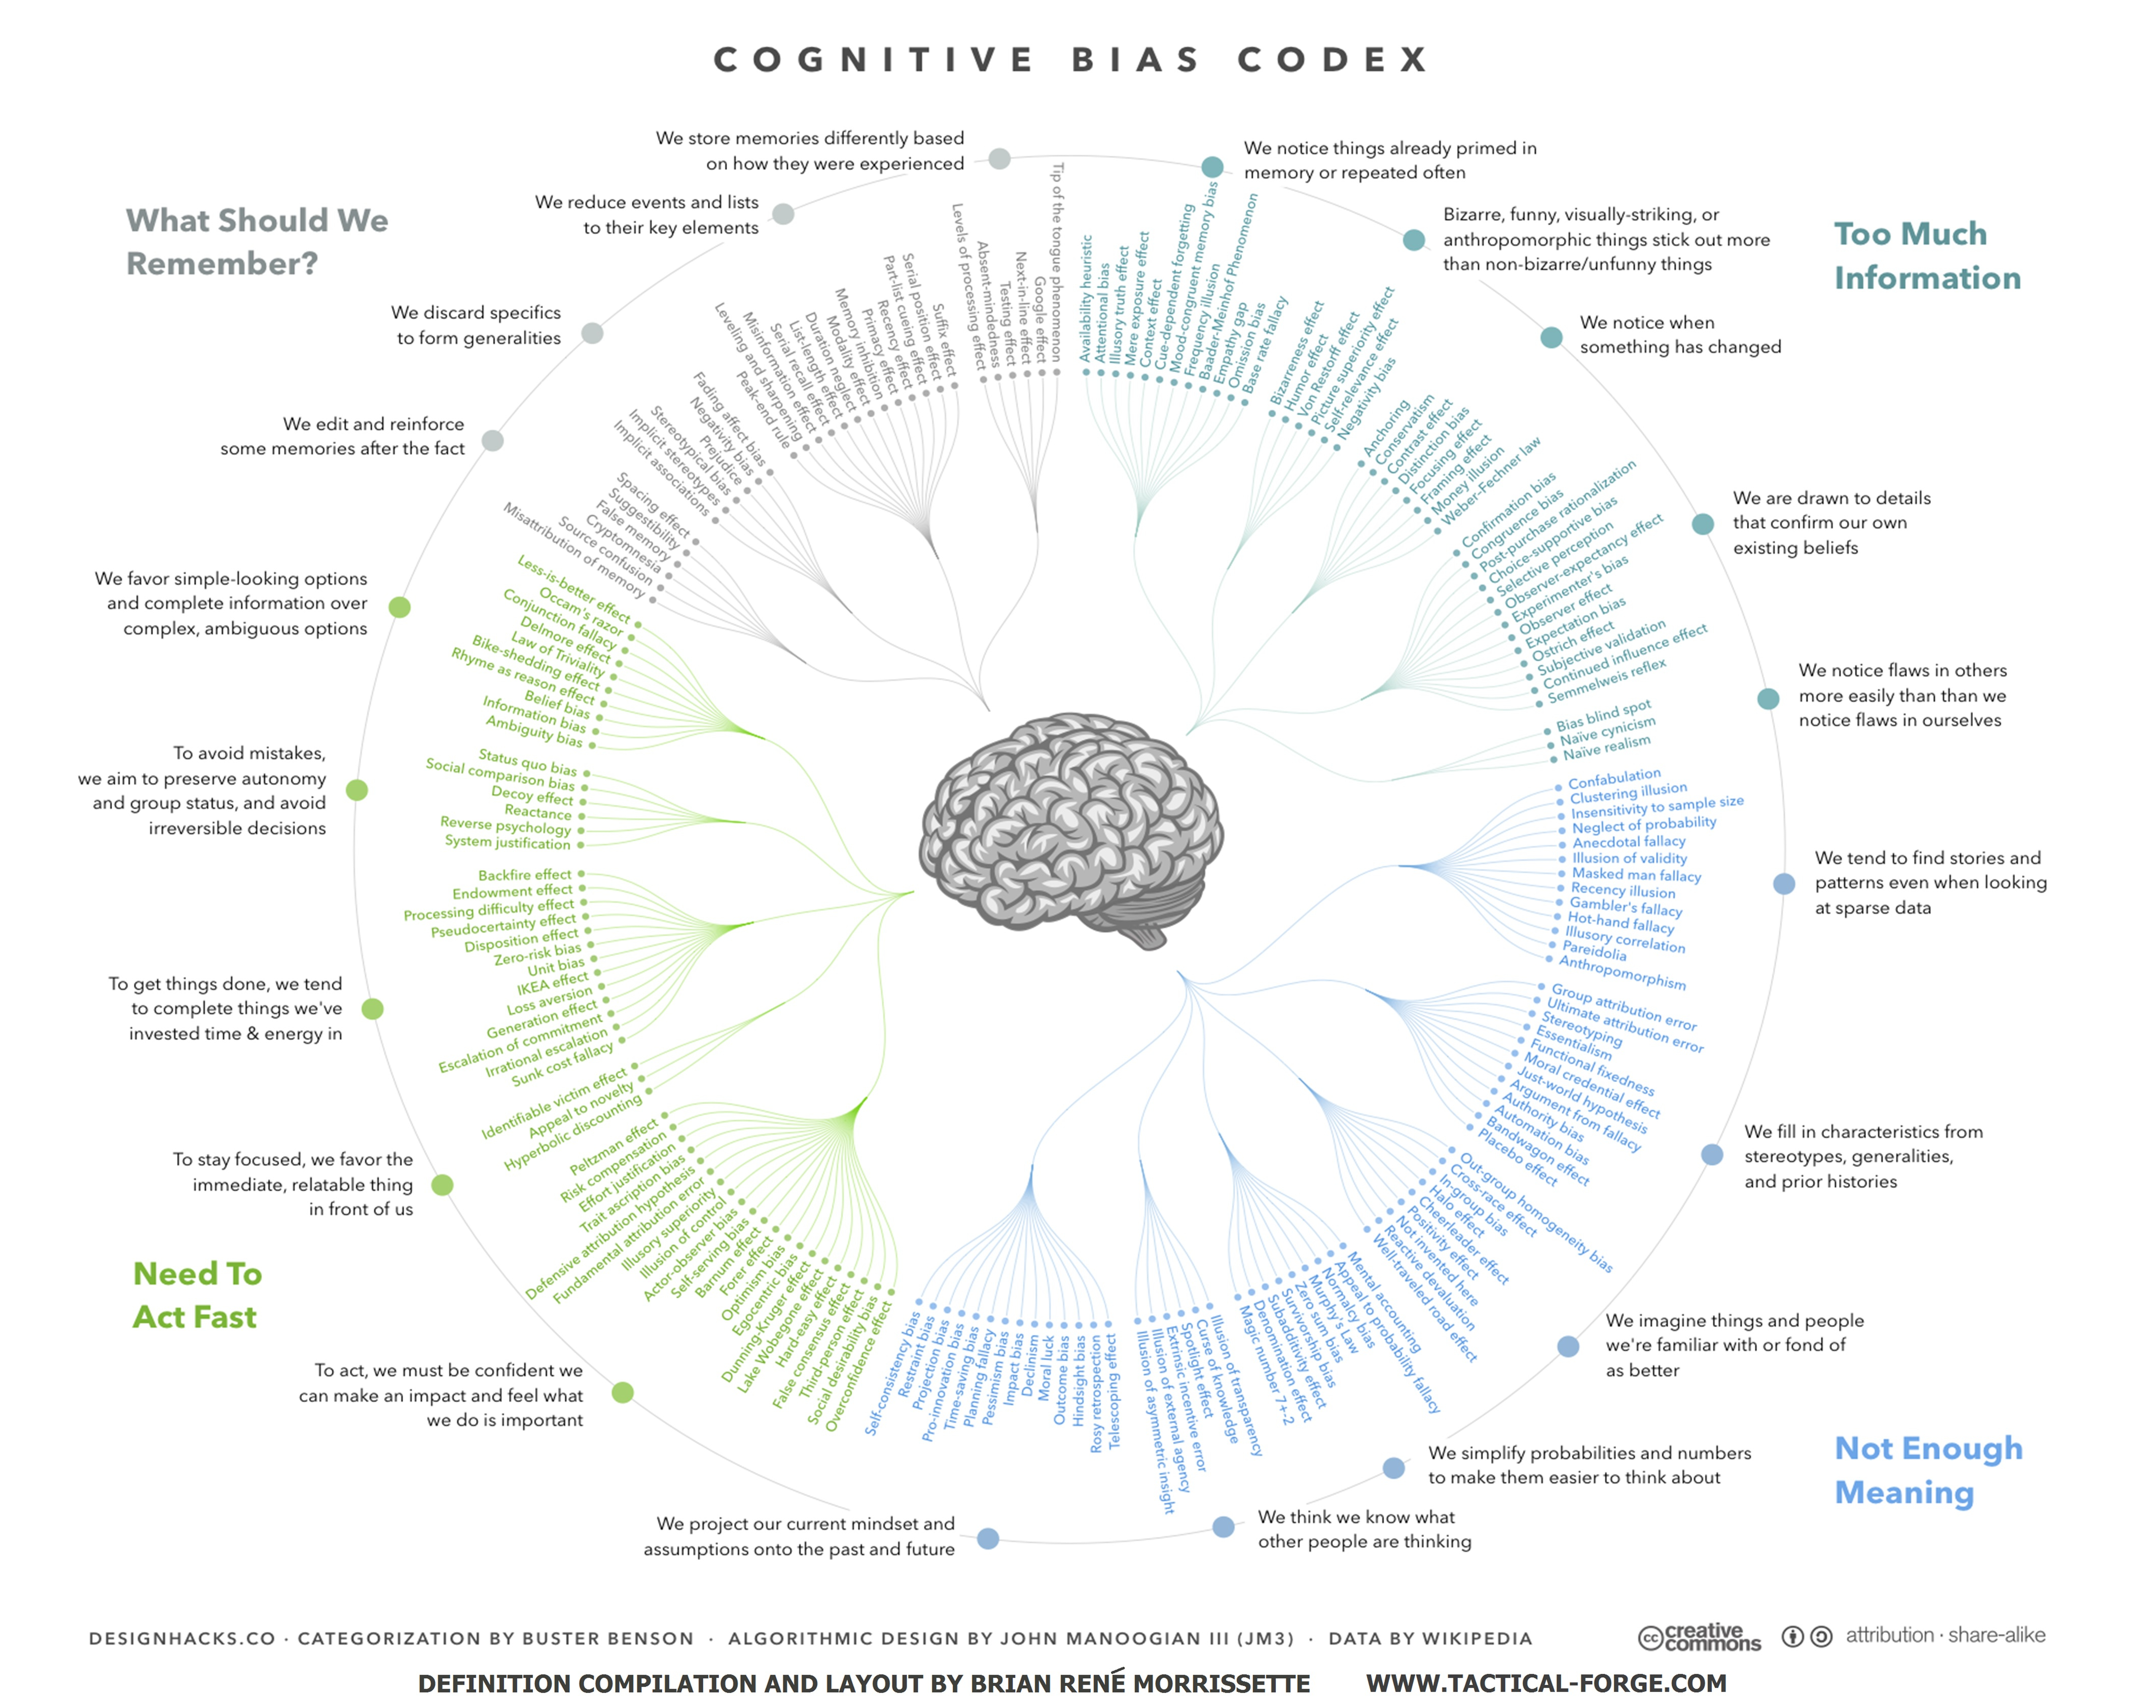
\includegraphics[width=\textwidth]{cogbias_0}
\end{frame}

% 
% \begin{frame}[c]{Denken, schnell und langsam}
%     \Large
%     \pause
%     % Das Gehirn arbeitet üblicherweise mit zwei verschiedenen Systemen
%     \begin{itemize}
%     \item System I - schnelles Denken
%     \newline
%     \pause
%     \item System II - langsames Denken
%     \end{itemize}
% \end{frame}
% 
